%!TEX TS-program = Xelatex  
%!TEX encoding = UTF-8 Unicode  
  
  
\documentclass[12pt]{article}  
\usepackage{geometry}  
\geometry{letterpaper}  
  
\usepackage{fancyhdr} 
\usepackage{layout}
\addtolength{\hoffset}{-1.0cm} \addtolength{\textwidth}{2cm}
\addtolength{\voffset}{-1.0cm} \addtolength{\textheight}{2cm}
\usepackage[rgb]{xcolor}

\usepackage{cite}
\makeatletter
\def\@cite#1#2{\textsuperscript{[{#1\if@tempswa , #2\fi}]}}
\makeatother

\usepackage{listings}
\definecolor{dkgreen}{rgb}{0,0.6,0}
\definecolor{gray}{rgb}{0.5,0.5,0.5}
\definecolor{bcol}{rgb}{0.85,0.85,0.85}
\definecolor{mauve}{rgb}{0.58,0,0.82}
\definecolor{mygray}{gray}{.9}
\definecolor{mypink}{rgb}{.99,.91,.95}
\definecolor{mycyan}{cmyk}{.3,0,0,0}

\lstset{ %
language=python,                % the language of the code
basicstyle=\footnotesize,       % the size of the fonts that are used for the code
numbers=left,                   % where to put the line-numbers
numberstyle=\tiny\color{gray},  % the style that is used for the line-numbers
stepnumber=1,                   % the step between two line-numbers. If it's 1, each line
                                % will be numbered
numbersep=5pt,                  % how far the line-numbers are from the code
backgroundcolor=\color{bcol},   % choose the background color. You must add \usepackage{color}
showspaces=false,               % show spaces adding particular underscores
showstringspaces=false,         % underline spaces within strings
showtabs=false,                 % show tabs within strings adding particular underscores
frame=shadowbox,                % adds a frame around the code
rulecolor=\color{black},        % if not set, the frame-color may be changed on line-breaks within not-black text (e.g. commens (green here))
tabsize=2,                      % sets default tabsize to 2 spaces
captionpos=t,                   % sets the caption-position to bottom
breaklines=true,                % sets automatic line breaking
breakatwhitespace=false,        % sets if automatic breaks should only happen at whitespace
title=\lstname,                     % show the filename of files included with \lstinputlisting;
                                    % also try caption instead of title
keywordstyle=\color{blue},          % keyword style
commentstyle=\color{dkgreen},       % comment style
stringstyle=\color{mauve},          % string literal style
escapeinside=``,                    % if you want to add LaTeX within your code
morekeywords={LONG64,LONGLONG,bool}                % if you want to add more keywords to the set
}



\usepackage{flushend, cuted} %

\usepackage{indentfirst,latexsym,bm}
\usepackage{amsmath,amssymb,amsfonts}
\usepackage{pifont} 
\usepackage{fontspec,xltxtra,xunicode}  
\defaultfontfeatures{Mapping=tex-text}  

\usepackage{algorithmic}
\usepackage[noend, ruled, linesnumbered]{algorithm2e}
\setromanfont{华文宋体} %设置中文字体  
\XeTeXlinebreaklocale “zh”  
\XeTeXlinebreakskip = 0pt plus 1pt minus 0.1pt %文章内中文自动换行  
  
 \setlength{\columnsep}{3em}          %设置分栏间隔
\setlength{\parindent}{2em}          %设置段首缩进量
\renewcommand{\baselinestretch}{1.2} %重设行距     
 \usepackage{graphicx}
\usepackage{cite}
\newcommand{\red}[1]{  \textcolor{red}  {#1}}   %红色\makeatletter
\newcommand{\blue}[1]{ \textcolor{blue} {#1}}   %蓝色\def\@cite#1#2{\textsuperscript{[{#1\if@tempswa , #2\fi}]}}
\newcommand{\green}[1]{\textcolor{green}{#1}}   %绿色\makeatother


% ----------------------------------------------------------------
\vfuzz2pt % Don't report over-full v-boxes if over-edge is small
\hfuzz2pt % Don't report over-full h-boxes if over-edge is small

%%--------------------------------------------------
%% 图片文件路径
%%--------------------------------------------------
\graphicspath{{Figures/}}


% MATH -----------------------------------------------------------
\DeclareMathOperator{\diag}{diag}
\DeclareMathOperator{\rank}{rank}
\DeclareMathOperator{\vecm}{vec}
\DeclareMathOperator{\vecs}{vecs}

\newcommand{\mfloor}[1]{ \left\lfloor {#1} \right\rfloor }
\newcommand{\mpair}[2]{ \left\langle {#1}, {#2} \right\rangle}


\renewcommand{\bf}[1]{\mathbf{#1}}
\renewcommand{\vec}[1]{\bm{#1}}    %向量, 黑斜体
\newcommand{\mat}[1]{\bm{#1}}    %矩阵
\newcommand{\dif}{\mathrm{d}}
\newcommand{\me} {\mathrm{e}}
\newcommand{\mi} {\mathrm{i}}
\newcommand{\vei} {\mathrm{vec}}

\newcommand{\vecmat}[1]{\vecm{\left( #1 \right)}}
\newcommand{\vecsmat}[1]{\vecs{\left( #1 \right)}}
\newcommand{\vecasym}[1]{[#1]_\times}   % antisymmetric matrix from a vector
\newcommand{\id} {\mathbbm{1}}   % identity operator
\newcommand{\fracode}[2]{\frac{\dif {#1}}{\dif {#2}}}         % ordinary differential operator
\newcommand{\fracpde}[2]{\frac{\partial {#1}}{\partial {#2}}} % partial differential operator
\newcommand{\fracpderow}[2]{\partial {#1}/\partial {#2}}
\newcommand{\fracoderow}[2]{\dif {#1}/\dif {#2}}
\newcommand{\fracpdemix}[3]{\frac{\partial^2 {#1}}{\partial {#2} \partial {#3}}}
\newcommand{\lap}[2]{\frac{\partial^2 {#1}}{\partial {#2}^2}}
\newcommand{\laprow}[2]{\partial^2 {#1}/\partial {#2}^2}
\newcommand{\secode}[2]{\frac{\dif^2 {#1}}{\dif {#2}^2}}
\newcommand{\set}[1]{\left\{ #1 \right\}}
\newcommand{\abs}[1]{\left| #1 \right|}
\newcommand{\absvec}[1]{\left| \bf{#1} \right|}
\newcommand{\ket}[1]{|#1 \rangle}
\newcommand{\bra}[1]{\langle #1 |}
\newcommand{\braket}[2]{ \langle #1 | #2 \rangle}
\newcommand{\norm}[1]{\lVert #1 \rVert}
\newcommand{\normF}[1]{{\parallel #1 \parallel}_\textrm{F}}
\newcommand{\trsp}[1]{{#1}^\textsf{T}}
\newcommand{\inv}[1]{#1^{-1}}
\newcommand{\ginv}[1]{#1^+}    % Moore-Penrose (general) inverse
\newcommand{\tinv}[1]{{#1}^{-\textsf{T}}}


\newcommand{\ES}[3]{\mathbb{#1}^{{#2}\times {#3}}}               % Euclidean space
\newcommand{\PS}[3]{\mathbb{#1}^{{#2}\times{#3}}}      % projective space
% ----------------------------------------------------------------
\newfontfamily{\H}{微软雅黑}  
\newfontfamily{\E}{Arial}  


\newfontfamily{\TNR}{Times New Roman}  %设定新的字体快捷命令  
\title{{\H Weekly Report of Research Work\\ }\quad {WR-ABS-TEMP-2015A-No.008}}
\author{汤吉(Ji TANG)\\
               Number: WR-ABS-TEMP-2015A,  E-mail: tangji08@hotmail.com \\
        Date: 11/3/2016 - 17/1/2016}
        \date{January 17, 2016}

  
 %%*************************************************
%%  打印 标题, 作者, 日期等内容
%%*************************************************
\begin{document}  
\maketitle
%%*********************************************
%% 设置页眉与页脚
%%*********************************************
\pagestyle{fancy}
\fancyhead[LO,RE]{\leftmark} % clear all fields
\fancyhead[RO,LE]{WR-ABS-TEMP-2015A-No.008-TJx}   %  请设置正确的个人文档编号



\fancyfoot[LO,RE]{SIAE}
\fancyfoot[RO,RE]{Ji Tang}
\renewcommand{\headrulewidth}{0.4pt}
\renewcommand{\footrulewidth}{0.4pt}



%%*************************************************
%% 显示内容目录
%%*************************************************
\tableofcontents 
\newpage
%%*************************************************
%% 正文部分
%%*************************************************
\section{\H Work}
\begin{enumerate}
	\item I have written a python program (including 13  functions) in order to plot the chart in the time slot you want .
	
	{\H Before the optimization}, it took {\H 3 minutes} to plot the chart from 20070103 to 20080801.
	
	And {\H after the optimization}, it took only {\H 3 seconds} to plot the same chart!
	\item I have studied "Econophysics" and "Basic random economics"
	\item I have tried to write a program to calculate the "Hurst Exponent"
\end{enumerate}

\section{\H The Python Program}
\subsection{\H Plot the file of the form ".txt"}
At first, I want to write a program to plot the data file for each year. So I need to transform the file into data list. The txt file just like this:

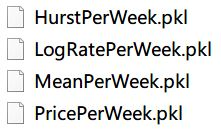
\includegraphics[width = 4.5in]{1.jpg}

What the program read is just about 

"/xf/xef20150101,231700,1186.4,1186.5,1186.4,1186.5,4"

\begin{lstlisting}
#This function will read the file and transform it into data
def file2data(filename):
    Date = []
    Time = []
    Price = []
    fr = open(filename)  # Load the data
    for line in fr.readlines():
        lines = line.strip()  # Strip the beginning and the end blank
        listFromLine = lines.split(',')  # Separate each line by '\t'
        Datelist = re.findall('\d', listFromLine[0])  # Find out the useful number data
        Dateint = int(string.join(Datelist, ''))  # Rejoin the characters
        Date.append(Dateint)  # Get the evaluate of each person
        Time.append(listFromLine[1])
        Price.append(float(listFromLine[2]))
    return Date, Time, Price
\end{lstlisting}

Then this program will split it by "," and read the integers only and finally return three list in the forms of "20150101", "231700" and "1186.4".

Next, I need to calculate the distance between two data, and the distance need to be uniformly defined. In my opinion, we can transform the time into the fractional part of the day and calculate the distance of two "float days". So I write two functions, the first one will calculate the number of days between two days, and the second one will give a sequence number for each data based on the first data (the first data is set "0").
\begin{lstlisting}
# To creat a funtion calculating the numbers of days between two dates
def datediff(beginDate, endDate):
    format = "%Y%m%d"
    # Translate the string to time form
    bd = time.strptime(beginDate, format)
    ed = time.strptime(endDate, format)
    # Translate the time form to date form
    bd = datetime.datetime(bd[0], bd[1], bd[2], bd[3], bd[4], bd[5])
    ed = datetime.datetime(ed[0], ed[1], ed[2], ed[3], ed[4], ed[5])
    oneday = datetime.timedelta(days = 1)
    count = 0
    while bd != ed:
        ed = ed-oneday
        count += 1
    return count
\end{lstlisting}

\begin{lstlisting}
#This function will set the first data time as the "0" time and format the following data based on this time
def time2number(Date, Time):
    NumbersOfLines = len(Date) # Get the number of the lines
    index1 = 0
    index2 = 0
    day = np.zeros(NumbersOfLines)
    hourp = np.zeros(NumbersOfLines)
    #Set the "0" moment
    Date0 = str(Date[0])
    number0 = Time[0]
    hour0 = float(number0[0: 2]) + float(number0[2: 4]) / 60
    for date in Date:
        datestring = str(date)
        day[index1] = datediff(Date0, datestring)
        index1 += 1
    for days in Time:
        hour = float(days[0: 1]) + float(days[2: 3]) / 60 +float(days[4:5]) / 3600
        hourp = float(hour - hour0) / 24
        index2 += 1
    day = np.array(day)
    return (day + hourp)
\end{lstlisting}

Finally, We can use the data we get to plot the file.
\begin{lstlisting}
def plotforextxt(filename):
    Date, Time, Price = file2data(filename)
    Day = time2number(Date, Time)
    fp = filename[0: 6] + "_" + str(Date[0]) + "_" + str(Date[-1])

    #**********************************************************
    fig = plt.figure(figsize=(8, 6), dpi=84, facecolor="white")
    axes = plt.subplot(111)
    axes.cla() # Clear all the information in the coordinate
    # Assign the font of the picture
    font = {'family' : 'serif',
            'color'  : 'darkred',
          'weight' : 'normal',
           'size'   : 16,
          }
    #**********************************************************
    plt.plot(Day, Price)
    # Configurate the scale of the coordinate
    ax=plt.gca()
    ax.set_xticks(np.linspace(0, Day[-1], 10))
    #ax.set_xticklabels( ('0', '500', '1000', '1500', '2000'))
    ax.set_yticks(np.linspace(min(Price), max(Price), 10))
    #ax.set_yticklabels( ('500', '800', '1100', '1400', '1700','2000'))
    # Configurate the labels
    xlabel = "The day from "+str(Date[0])
    ylabel = "The price of the international gold"
    ax.set_ylabel(ylabel, fontdict = font)
    ax.set_xlabel(xlabel, fontdict = font)
    # Configurate the title
    titleStr = 'The Price of Gold '
    plt.title(titleStr)
    figname = fp+'.png'
    plt.savefig(figname)
    #plt.clf() # Clear the chart

    #plt.show()
    print('ALL -> Finished OK')

    plt.show()
\end{lstlisting}

For example, if we choose to plot the chart of 2008:
\begin{lstlisting}
import FkNN
FkNN.plotforextxt("XAUUSD_2008.txt")
\end{lstlisting}

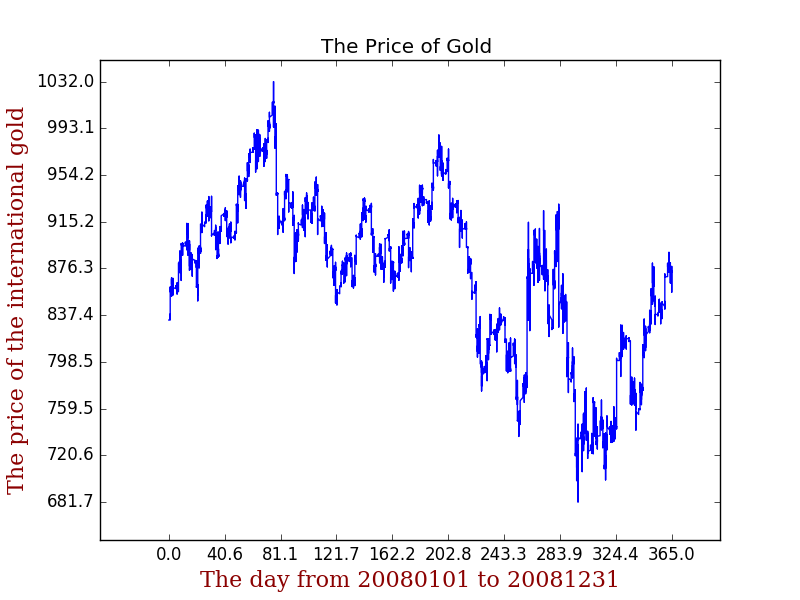
\includegraphics[width = 4.5in]{2.png}

\subsection{\H Plot the chart of the period you want}
Then I want to plot the chart whenever you need. So I write two new functions:
\begin{lstlisting}
def input2data(forextype, startdate, enddate):
    startyear = startdate[0: 4]
    startmonth = startdate[4: 8]
    endyear = enddate[0: 4]
    endmonth = enddate[4: 8]
    startfilename = forextype + "_" + startyear + ".txt"
    endfilename = forextype + "_" + endyear + ".txt"
    returndate = []
    returntime = []
    returnprice = []
    date1, time1, price1 = file2data(startfilename)
    date2, time2, price2 = file2data(endfilename)

    startyear = int(startyear)
    endyear = int(endyear)
    starttime = int(str(startyear) + str(startmonth))
    endtime = int(str(endyear) + str(endmonth))

    # This part will select a closely date if the input date isn't the work day.
    startindex = -1
    endindex = -1
    while (startindex == -1):
        try:
            startindex = date1.index(starttime)
        except:
            starttime += 1
    while (endindex == -1):
        try:
            endindex = date2.index(endtime)
        except:
            endtime -= 1

    if (startyear == endyear):
        for index in range(startindex, endindex):
            returndate.append(date1[index])
            returntime.append(time1[index])
            returnprice.append(price1[index])
    elif (startyear < endyear):
        for index in range(startindex, len(date1)):
            returndate.append(date1[index])
            returntime.append(time1[index])
            returnprice.append(price1[index])
        startyear += 1
        while (startyear < endyear):
            startfilename = forextype + "_" + str(startyear) + ".txt"
            datewhole, timewhole, pricewhole = file2data(startfilename)
            for index in range(0, len(datewhole)):
                returndate.append(index)
                returntime.append(index)
                returnprice.append(index)
            startyear += 1
        for index in range(0, endindex):
            returndate.append(date2[index])
            returntime.append(time2[index])
            returnprice.append(price2[index])
    return returndate, returntime, returnprice
\end{lstlisting}

\begin{lstlisting}
def plotforexdata(Date, Time, Price, name):
    Day = time2number(Date, Time)
    fp = name + "_" + str(Date[0]) + "_" + str(Date[-1])

    #**********************************************************
    fig = plt.figure(figsize=(8, 6), dpi=84, facecolor="white")
    axes = plt.subplot(111)
    axes.cla() # Clear all the information in the coordinate
    # Assign the font of the picture
    font = {'family' : 'serif',
            'color'  : 'darkred',
          'weight' : 'normal',
           'size'   : 16,
          }
    #**********************************************************
    plt.plot(Day, Price)
    # Configurate the scale of the coordinate
    ax=plt.gca()
    ax.set_xticks(np.linspace(0, Day[-1], 10))
    #ax.set_xticklabels( ('0', '500', '1000', '1500', '2000'))
    ax.set_yticks(np.linspace(min(Price), max(Price), 10))
    #ax.set_yticklabels( ('500', '800', '1100', '1400', '1700','2000'))
    # Configurate the labels
    xlabel = "The day from " + str(Date[0]) + " to " + str(Date[-1])
    ylabel = "The price of the international gold"
    ax.set_ylabel(ylabel, fontdict = font)
    ax.set_xlabel(xlabel, fontdict = font)
    # Configurate the title
    titleStr = 'The Price of Gold '
    plt.title(titleStr)
    figname = fp+'.png'
    plt.savefig(figname)
    #plt.clf() # Clear the chart

    #plt.show()
    print('ALL -> Finished OK')

    plt.show()
\end{lstlisting}

Then, if we want to plot the data from January 3, 2007 to June 31, 2008.

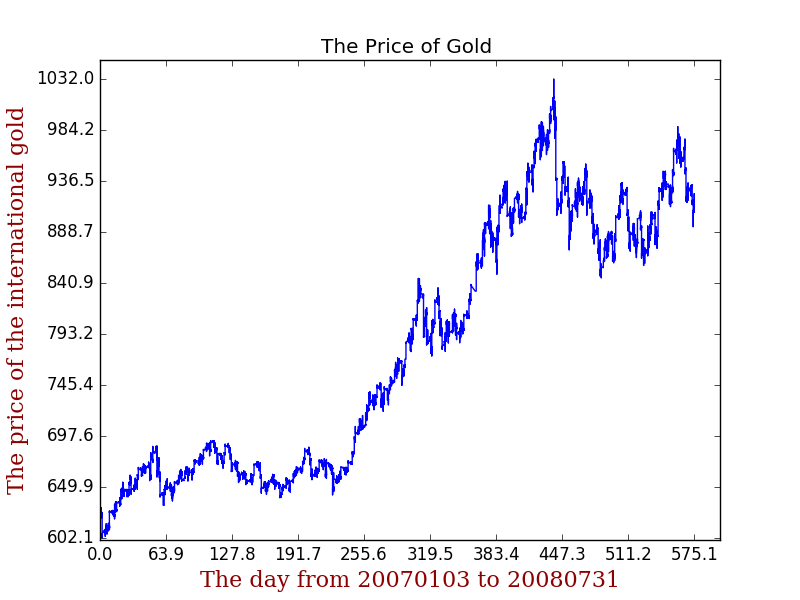
\includegraphics[width = 4.5in]{3.png}

\H{It does work, but it took about 3 minutes to draw this chat! It's too slowly!}

\subsection{\H The optimizing}
Because of its wasting of too much time, I have optimized the program by making the series of new data with UTC in each line of file. And I can get a series of new data with the beginning of "UTC" by the following function:
\begin{lstlisting}
# code: UTF-8
import re
import string
import numpy as np
import datetime
import time
import matplotlib.pyplot as plt

#This function will read the file and translate it to data
def file2data(filename):
    Date = []
    Time = []
    Price = []
    fr = open(filename)  # Load the data
    for line in fr.readlines():
        lines = line.strip()  # Strip the beginning and the end blank
        listFromLine = lines.split(',')  # Separate each line by '\t'
        Datelist = re.findall('\d', listFromLine[0])  # Find out the useful number data
        Dateint = int(string.join(Datelist, ''))  # Rejoin the characters
        Date.append(Dateint)  # Get the evaluate of each person
        Time.append(listFromLine[1])
        Price.append(float(listFromLine[2]))
    return Date, Time, Price


def str2UTC(timestr):
    return str(int(time.mktime(time.strptime(timestr, "%Y%m%d%H%M%S"))))


def writeUTC(Date, Time ,Price , filename):
    returnfile = open("UTC"+filename, "w")
    for index in range(len(Date)):
        returnfile.write(str2UTC((Date[index])+str(Time[index])) + "," + str(returnUTC[index]) + "," + str(Price[index]) + "\n")
    returnfile.close()
\end{lstlisting}

The new data the program had set up are:

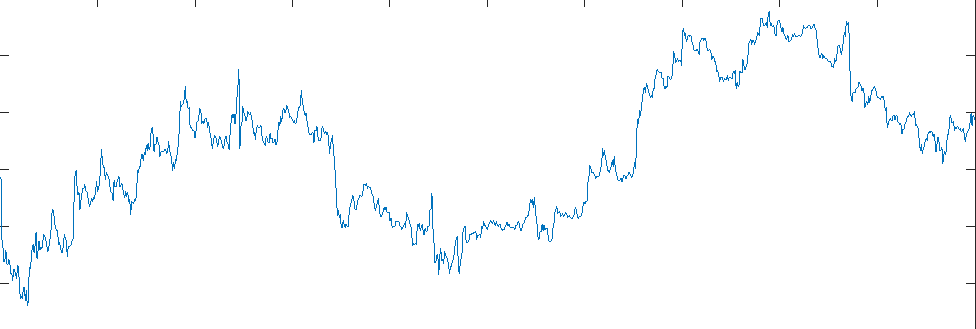
\includegraphics[width = 4.5in]{2.jpg}

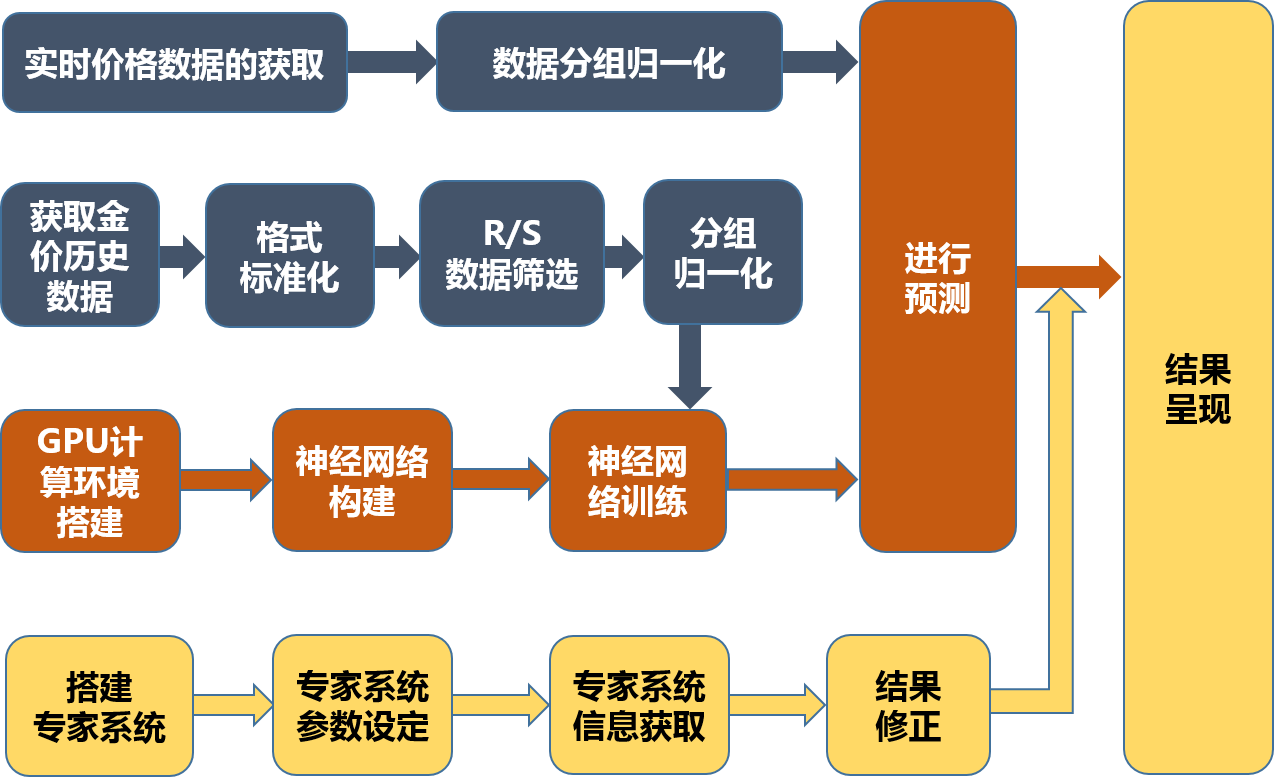
\includegraphics[width = 4.5in]{3.jpg}

And then I wrote the new functions to plot this kind of data:

\begin{lstlisting}
def UTCfile2data(filename):
    Time = []
    UTC = []
    Price = []
    fr = open(filename)  # Load the data
    for line in fr.readlines():
        lines = line.strip()  # Strip the beginning and the end blank
        listFromLine = lines.split(',')  # Separate each line by '\t'
        Time.append(listFromLine[0])
        UTC.append(float(listFromLine[1]))
        Price.append(float(listFromLine[2]))
    return Time, UTC, Price
\end{lstlisting}

The first function will transform the new UTC data into python data .

\begin{lstlisting}
def plotUTCforexdata(Time, UTC, Price, name):
    fp = name + "_" + str(Time[0][0:8]) + "_" + str(Time[-1][0:8])

    #**********************************************************
    fig = plt.figure(figsize=(8, 6), dpi=84, facecolor="white")
    axes = plt.subplot(111)
    axes.cla() # Clear all the information in the coordinate
    # Assign the font of the picture
    font = {'family' : 'serif',
            'color'  : 'darkred',
          'weight' : 'normal',
           'size'   : 16,
          }
    #**********************************************************
    plt.plot(UTC, Price)
    # Configurate the scale of the coordinate
    ax = plt.gca()
    interval = int(len(Price) / 5)
    ax.set_xticks(np.linspace(UTC[0], UTC[-1], 5))
    ax.set_xticklabels( (Time[0][0:8], Time[interval][0:8], Time[2*interval][0:8], Time[3*interval][0:8], Time[-1][0:8]))
    ax.set_yticks(np.linspace(min(Price), max(Price), 8))
    #ax.set_yticklabels( ('500', '800', '1100', '1400', '1700','2000'))
    # Configurate the labels
    xlabel = "The day from " + str(Time[0][0:8]) + " to " + str(Time[-1][0:8])
    ylabel = "The price of the international gold"
    ax.set_ylabel(ylabel, fontdict=font)
    ax.set_xlabel(xlabel, fontdict=font)
    ax.grid(True)
    # Configurate the title
    titleStr = 'The Price of Gold '
    plt.title(titleStr)
    figname = fp+'.png'
    try:
        os.mkdir('../Pictures/')
    except:
        plt.savefig('../Pictures/'+ figname)
    # savefig('../figures/contour_ex.png',dpi=48)
    #plt.clf() # Clear the chart

    #plt.show()
    print('ALL -> Finished OK')

    plt.show()
\end{lstlisting}

The second function will plot the new data with UTC time, and it can finally translate the UTC time into normal time for axis x.

For example, if we want to plot the Gold Price Chart from 20070103 to 20080801 again.

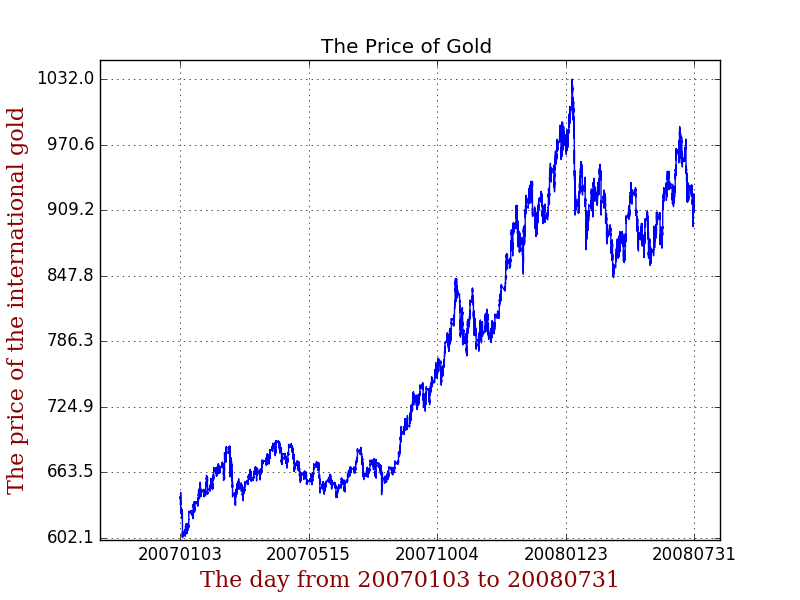
\includegraphics[width = 4.5in]{4.png}

It took me just 3 seconds!!! It works as 60 times quicker as the first time! 

\section{\H The Econophysices}
\subsection{\H 对数收益率、随机游走、峰度}
不同的交易资产有着相似的规律[Pagan(1996), Matteo, Aste, and Dacorogna(2005)]
由于通常认为股价波动服从几何布朗运动,对数收益率也就自然成为了最常见的分析对象[Hull(2008)]. S(t) = lnP(t+dt) – lnP(t). 该方法的优点是,无需贴现因子,尺度变化的平均修正已被考虑在内.

随机游走(random walk)是一类最简单的随机过程,在数量金融领域有重要的理论意义与应用价值,其数学统计模型最早由英国数学家卡尔·皮尔逊(Karl Pearson, 1857-1936)在1905年提出
峰度$k=\frac{\sum^{N}_{i=1}[S(t_i)-\mu]^4}{\sigma^4}$

正态分布的峰度k=3,对于股票收益率的大量实证研究,均得到k大于3的结论

\subsection{\H Hurst exponent}
The Hurst exponent is used as a measure of long-term memory of time series. It relates to the autocorrelations of the time series, and the rate at which these decrease as the lag between pairs of values increases. Studies involving the Hurst exponent were originally developed in hydrology for the practical matter of determining optimum dam sizing for the Nile river's volatile rain and drought conditions that had been observed over a long period of time. The name "Hurst exponent", or "Hurst coefficient", derives from Harold Edwin Hurst (1880–1978), who was the lead researcher in these studies; the use of the standard notation H for the coefficient relates to his name also.

The Hurst exponent is referred to as the "index of dependence" or "index of long-range dependence". It quantifies the relative tendency of a time series either to regress strongly to the mean or to cluster in a direction A value H in the range 0.5–1 indicates a time series with long-term positive autocorrelation, meaning both that a high value in the series will probably be followed by another high value and that the values a long time into the future will also tend to be high. A value in the range 0 – 0.5 indicates a time series with long-term switching between high and low values in adjacent pairs, meaning that a single high value will probably be followed by a low value and that the value after that will tend to be high, with this tendency to switch between high and low values lasting a long time into the future. A value of H=0.5 can indicate a completely uncorrelated series, but in fact it is the value applicable to series for which the autocorrelations at small time lags can be positive or negative but where the absolute values of the autocorrelations decay exponentially quickly to zero. This in contrast to the typically power law decay for the 0.5 < H < 1 and 0 < H < 0.5 cases.

\subsubsection{Definition}
The Hurst exponent, H, is defined in terms of the asymptotic behaviour of the rescaled range as a function of the time span of a time series as follows

\subsubsection{Estimating the exponent}
To estimate the Hurst exponent, one must first estimate the dependence of the rescaled range on the time span n of observation. A time series of full length N is divided into a number of shorter time series of length n = N, N/2, N/4, ... The average rescaled range is then calculated for each value of n.
For a (partial) time series of length n, $X=X_1,X_2,..., X_n $ , the rescaled range is calculated as follows:

1. Calculate the mean
$$m=\frac{1}{n} \sum_{i=1}^{n} X_i$$

2. Create a mean-adjusted series
$$Y_t=X_{t}-m \quad \text{for}~~ t=1,2, \dots ,n $$

3. Calculate the cumulative deviate series Z
$$Z_t= \sum_{i=1}^{t} Y_{i} \quad \text{ for } t=1,2, \dots ,n $$

4. Compute the range R
$$R(n) =\operatorname{max}\left (Z_1, Z_2, \dots, Z_n \right )- \operatorname{min}\left (Z_1, Z_2, \dots, Z_n \right ). $$

5. Compute the standard deviation S
$$S(n)= \sqrt{\frac{1}{n} \sum_{i=1}^{n}\left ( X_{i} - m \right )^{2}}$$

6. Calculate the rescaled range R(n)/S(n) and average over all the partial time series of length n.

The Hurst exponent is estimated by fitting the power law $\operatorname{E} \left [ \frac{R(n)}{S(n)} \right ]=C n^H$ to the data. This can be done by plotting the logarithm of $\operatorname{E} \left [ \frac{R(n)}{S(n)} \right ] $as a function of$ \log n$, and fitting a straight line; the slope of the line gives H. Such a graph is called a pox plot. However, this approach is known to produce biased estimates of the power-law exponent. A more principled approach fits the power law in a maximum-likelihood fashion.

There are number of alternative techniques. Namely, DFA, Periodogram regression, aggregated variances, local Whittle's estimator, wavelet analysis, both in the time domain and frequency domain.

\subsubsection{Generalized exponent}
The basic Hurst exponent can be related to the expected size of changes, as a function of the lag between observations, as measured by $E(|X_{t+1}-X_t|^2)$. For the generalized form of the coefficient, the exponent here is replaced by a more general term, denoted by q.

There are a variety of techniques that exist for estimating H, however assessing the accuracy of the estimation can be a complicated issue. Mathematically, in one technique, the Hurst exponent can be estimated such that:
$$H_q = H(q)$$
for a time series
$$g(t) (t = 1, 2,...)$$
may be defined by the scaling properties of its structure functions $S_q(\tau)$:
$$S_q = \langle |g(t + \tau) - g(t)|^q \rangle_t \sim \tau^{qH(q)} $$

where q > 0, $\tau$ is the time lag and averaging is over the time window

$$t \gg \tau$$

usually the largest time scale of the system.

Practically, in nature, there is no limit to time, and thus H is non-deterministic as it may only be estimated based on the observed data; e.g., the most dramatic daily move upwards ever seen in a stock market index can always be exceeded during some subsequent day.

H is directly related to fractal dimension, D, where 1 < D < 2, such that D = 2 - H. The values of the Hurst exponent vary between 0 and 1, with higher values indicating a smoother trend, less volatility, and less roughness.

In the above mathematical estimation technique, the function H(q) contains information about averaged generalized volatilities\red{(波动系数)} at scale $\tau$ (only q = 1, 2 are used to define the volatility). In particular, the $H_1$ exponent indicates persistent $(H_1 > \frac{1}{2})$ or antipersistent\red{(反持久性效应)} $(H_1 < \frac{1}{2})$ behavior of the trend.

For the BRW (brown noise, $\frac{1}{f^2}$) one gets

$$Hq = \frac{1}{2}$$

and for pink noise ($\frac{1}{f}$)

$$Hq = 0$$

The Hurst exponent for white noise is dimension dependent, and for 1D and 2D it is

$$H^{1D}_q = -\frac{1}{2}, H^{2D}_q = -1$$

For the popular Lévy stable processes and truncated Lévy processes with parameter α it has been found that

$H_q = q/\alpha$ for $q < \alpha$ and $H_q = 1$ for $q \le \alpha$

A method to estimate H(q) from non-stationary time series is called detrended fluctuation analysis\red{(去趋势波动分析)}. When H(q) is a non-linear function of q the time series is a multifractal system.

\subsubsection{The code for calculating the Hurst Exponent}
\begin{lstlisting}
__author__ = 'Jojo'
import numpy as np
import math


def RS(Price):
    if len(Price) < 2:
        return 0
    Price = np.array(Price)
    n = len(Price)
    m = np.mean(Price)
    Y = Price - m
    Z = np.arange(n, dtype=float)
    for i in range(n):
        Z[i] = sum(Y[:i])
    R = max(Z) - min(Z)
    S = np.sqrt(np.var(Price))
    return R / S

def Hurst(Price):
    n = len(Price)
    times = int(math.log(n))
    x = []
    y = []
    price = Price
    for i in range(times):
        if(n > 4):
            x.append(n)
            y.append(RS(price[:n]))
        n = int(n / 2)
        Price_n = np.arange(n, dtype=float)
        for index in range(n):
            Price_n[index] = (price[2 * index] + price[2 * index + 1]) / 2
        price = Price_n
    print x, y
    k = np.polyfit(np.log(x), np.log(y), 1)
    return k[0]
\end{lstlisting}

\subsubsection{The code for ploting the Hurst Exponent}
\begin{lstlisting}
def data2hurst(UTC, Price, prange):
    p = len(UTC) / prange
    p = int(p)
    Hurstvalue = np.arange(0, p+1, dtype=float)
    for i in range(p):
        Hurstvalue[i] = Hurst(Price[i*prange:(i+1)*prange])
    Hurstvalue[p] = Hurst(Price[p*prange:])
    x = np.arange(p+1)
    return x, Hurstvalue


def plotprice_hurst(type, startime, endtime, prange):
    Time, UTC, Price = input2data("UTC" + type[-6:], startime, endtime)
    x, Hurstvalue = data2hurst(UTC, Price, prange)
    HurstTime = np.arange(len(x))
    for i in range(len(x)):
        HurstTime[i] = UTC[i * prange]
    fp = type[-6:] + "_" + str(Time[0][0:8]) + "_" + str(Time[-1][0:8])

    #**********************************************************
    fig = plt.figure(figsize=(8, 6), dpi=84, facecolor="white")
    axes = plt.subplot(211)
    axes.cla() # Clear all the information in the coordinate
    # Assign the font of the picture
    font = {'family' : 'serif',
            'color'  : 'darkred',
          'weight' : 'normal',
           'size'   : 16,
          }
    #**********************************************************
    plt.plot(UTC, Price)
    # Configurate the scale of the coordinate
    ax1 = plt.gca()
    interval = int(len(Price) / 5)
    ax1.set_xticks(np.linspace(UTC[0], UTC[-1], 5))
    ax1.set_xticklabels( (Time[0][0:8], Time[interval][0:8], Time[2*interval][0:8], Time[3*interval][0:8], Time[-1][0:8]))
    ax1.set_yticks(np.linspace(min(Price), max(Price), 8))
    #ax.set_yticklabels( ('500', '800', '1100', '1400', '1700','2000'))
    # Configurate the labels
    xlabel = "The day from " + str(Time[0][0:8]) + " to " + str(Time[-1][0:8])
    ylabel = "The international gold price"
    ax1.set_ylabel(ylabel, fontdict=font)
    ax1.set_xlabel(xlabel, fontdict=font)
    ax1.grid(True)

    #**********************************************************
    axes = plt.subplot(212)
    plt.plot(HurstTime, Hurstvalue)
    # Configurate the scale of the coordinate
    ax2 = plt.gca()
    ax2.set_xticks(np.linspace(HurstTime[0], HurstTime[-1], 5))
    ax2.set_xticklabels( (Time[0][0:8], Time[interval][0:8], Time[2*interval][0:8], Time[3*interval][0:8], Time[-1][0:8]))
    ax2.set_yticks(np.linspace(min(Hurstvalue), max(Hurstvalue), 8))
    #ax.set_yticklabels( ('500', '800', '1100', '1400', '1700','2000'))
    # Configurate the labels
    xlabel = "The day from " + str(Time[0][0:8]) + " to " + str(Time[-1][0:8])
    ylabel = "The Hurst Value"
    ax2.set_ylabel(ylabel, fontdict=font)
    ax2.set_xlabel(xlabel, fontdict=font)
    ax2.grid(True)

    # Configurate the title
    titleStr = 'The Price of Gold '
    plt.title(titleStr)
    figname = fp+'.png'
    try:
        os.mkdir('../Pictures/')
        plt.savefig('../Pictures/'+ figname)
    except:
        plt.savefig('../Pictures/'+ figname)
    # savefig('../figures/contour_ex.png',dpi=48)
    #plt.clf() # Clear the chart

    #plt.show()
    print('ALL -> Finished OK')

    plt.show()
\end{lstlisting}

\subsubsection{The result of the code}
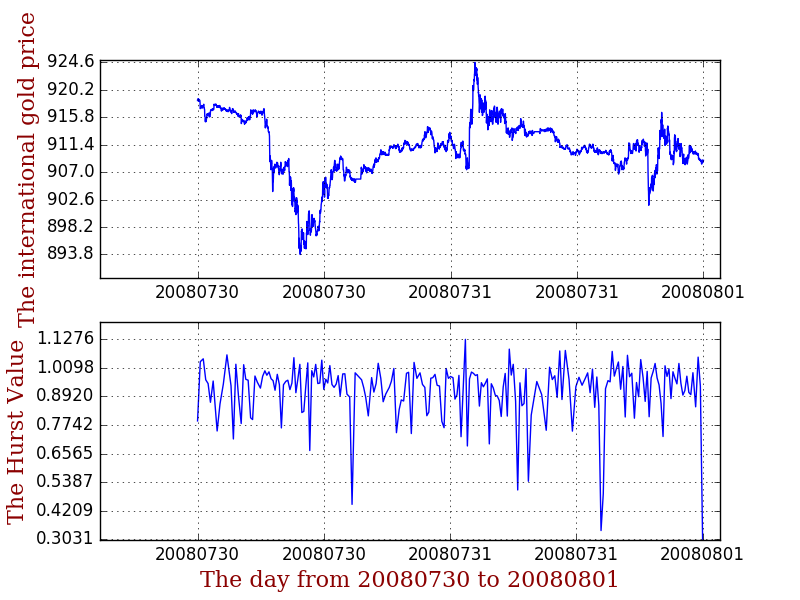
\includegraphics[width=4.5in]{6.png}


\subsection{\H 自更新向心布朗运动}
自更新向心布朗运动(Auto-Renewed Centripetal Brownian Motion)模型[周文超(2008),Yang, Zhou, and Huang(2012)]
假设一:供求原理
假设二:参与者的自我更新

以下是根据他的自更新向心布朗运动模型,编写的虚拟黄金走势程序以及图表:
\begin{lstlisting}
# -*- coding: utf-8 -*-
import numpy as np
import matplotlib.pyplot as plt

step = 0
numInMin = 60
p0 = 1000.00  # Set the initial price
p = p0
pE = p0
percent = 0.1
T = numInMin * 1000  #Total steps
uOrD = 0
rand = 0
crit = 0
ERROR = 0.001
memory = 10
history = np.tile(p0, (1, memory))
oneDay = numInMin * 240
recordFreq = numInMin * 1000
price = []
priceTemp = step / 60
printTemp = 0
totalstep = []

while(step < T):
    step += 1
    totalstep.append(step)
    price.append(p)
    crit = p / (2 * pE)
    rand = np.random.rand()
    if(rand < crit):
        uOrD = -1
    else:
        uOrD = 1
    p = p + uOrD * percent

    pE = np.mean(history)
    history = np.delete(history, 0)
    history = np.append(history, p)

fig = plt.figure(figsize=(8, 6), dpi=84, facecolor="white")
ax = plt.gca()
xlabel = "Day"
ylabel = "Price"
plt.title("Generatied by ARCH")
plt.plot(totalstep, price)
ax.grid(True)
figname = 'Brownian Motion Price.png'
try:
    os.mkdir('../Pictures/')
    plt.savefig('../Pictures/'+ figname)
except:
    plt.savefig('../Pictures/'+ figname)
plt.show()

\end{lstlisting}

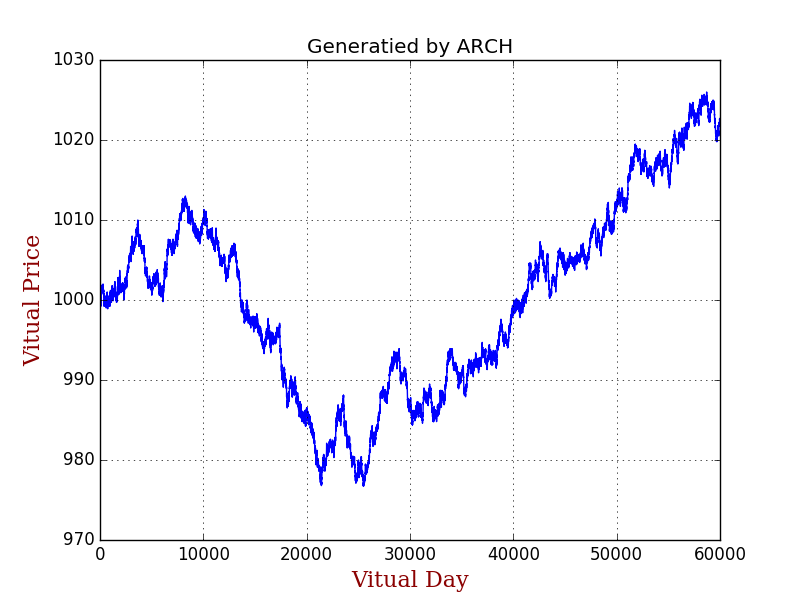
\includegraphics[width=4.5in]{5.png}


\subsection{\H 自相关系数与互相关系数}
自回归条件异方差模型(autoregressive conditional heteroskedasticity model, ARCH)用以描绘时间序列波动性的随时演变。

自相关系数(auto-correlation function)常见于信号处理与金融时间序列分析,用于表征同一序列不同时刻取值之间的相关程度。考察一个收益率时间序列S(t),其自协方差$Cov(\delta t)$定义为时间序列S(t)与其经过时间平移后的序列$S(t-\delta t)$之间的协方差。自协方差通过方差进行标准化之后,即成为自相关系数$\rho(\delta t)$。如下式表示 $$Cov(\delta t)=E\{[S(t)-\mu][S(t-\delta t)-\mu]\}$$ $$\rho(\delta t)=\frac{Cov(\delta t)}{\sigma}$$
其中,E(x)代表x的数学期望,$\mu$和$\sigma$分别为时间序列S(t)的平均值和标准差,自协方差$Cov(\delta t)$与自相关函数$\rho(\delta t)$均为平移时间间隔$\delta t$的函数。

互相关系数可应用于研究两个不同序列之间的相关性,例如两只股票的收益率时间序列之间的相关性、同一只股票的价格时间序列与交易量时间序列之间的相关性。
假设两个时间序列分别为$S_1(t)$与$S_2(t)$,则协方差$Cov(S_1,S_2)$与互相关函数$\rho(S_1,S_2)$分别定义为 $$COv(S_1,S_2)=E\{[S_1(t)-\mu_1][S_2(t)-\mu_2]\}$$
$$\rho(S_1,S_2)=\frac{Cov(S_1,S_2)}{\sigma_1 \sigma_2}$$

 

%%****************************************
%%  参考文献
%%****************************************
\bibliography{myreference}
\bibliographystyle{plain}
\end{document}  
